% Template for creating presentations
\documentclass[aspectratio=169]{beamer}

% --- Theme ---
\makeatletter
\def\input@path{{beamertheme-cleaneasy/theme/}}
\makeatother
\usepackage{beamerthemeCleanEasy}

% --- Essential packages ---
\usepackage{tikz}
\usepackage[american]{babel}
\usepackage{csquotes}
\usepackage[backend=biber, style=apa, sorting=nyt, doi=true, url=true]{biblatex}
\DeclareLanguageMapping{american}{american-apa}
\addbibresource{references.bib}  % Update with your .bib file
\setbeamertemplate{bibliography item}{\insertbiblabel}

% --- Tables and figures ---
\usepackage{booktabs}
\usepackage{array}
\setbeamertemplate{caption}[numbered]
\setbeamerfont{caption}{size=\footnotesize}
\setbeamercolor{caption name}{fg=gray}

% --- Graphics paths ---
\graphicspath{{figures/}{images/}}  % Update with your image directories

% --- Metadata ---
\title{Your Title Here}
\subtitle{Your Subtitle Here}
\author{Your Name}
\date{\today}
\institute{Your Institution}

\begin{document}

% Title
\begin{frame}
  \titlepage
\end{frame}

% ============================================================================
% JOB POSTING
% ============================================================================

\begin{frame}
  \frametitle{Join Our Team!}

  \begin{beamercolorbox}[wd=\textwidth,sep=0.4em,colsep=0pt]{block title}
    \textbf{We're Hiring: Research Position in Language Production Lab}
  \end{beamercolorbox}

  \vspace{1em}

  \textbf{What we do:}
  \begin{itemize}
    \item Study how humans and AI learn language
    \item Combine computational modeling with linguistic theory
    \item Use cutting-edge NLP techniques to understand cognition
  \end{itemize}

  \vspace{1em}

  \textbf{Who we're looking for:}
  \begin{itemize}
    \item Interest in language, AI, or cognitive science
    \item Programming experience (Python preferred)
    \item Enthusiasm for interdisciplinary research
  \end{itemize}

  \vspace{1em}

  \begin{beamercolorbox}[wd=\textwidth,sep=0.3em,colsep=0pt]{block body}
    \textbf{Interested?} Contact us at: [your-email@institution.edu]
  \end{beamercolorbox}
\end{frame}

% ============================================================================
% ATKINSON & SHIFFRIN MODEL OF MEMORY
% ============================================================================

\begin{frame}
  \frametitle{The Atkinson-Shiffrin Model of Memory}

  \begin{beamercolorbox}[wd=\textwidth,sep=0.4em,colsep=0pt]{block title}
    \textbf{A Classic Framework for Understanding Memory (1968)}
  \end{beamercolorbox}

  \vspace{1em}

  \textbf{Key Insight:}
  \begin{itemize}
    \item Memory is not a single system
    \item Information flows through multiple stages
    \item Each stage has different properties and purposes
  \end{itemize}

  \vspace{1em}

  \textbf{The Three Stages:}
  \begin{enumerate}
    \item \textbf{Sensory Memory} - Brief, high-capacity storage of raw sensory input
    \item \textbf{Short-Term Memory} - Limited capacity working memory
    \item \textbf{Long-Term Memory} - Unlimited capacity permanent storage
  \end{enumerate}

  \vspace{1em}

  \begin{beamercolorbox}[wd=\textwidth,sep=0.3em,colsep=0pt]{block body}
    Also known as the "Modal Model" - became the dominant framework for decades
  \end{beamercolorbox}
\end{frame}

\begin{frame}
  \frametitle{How the System Works}

  \begin{center}
  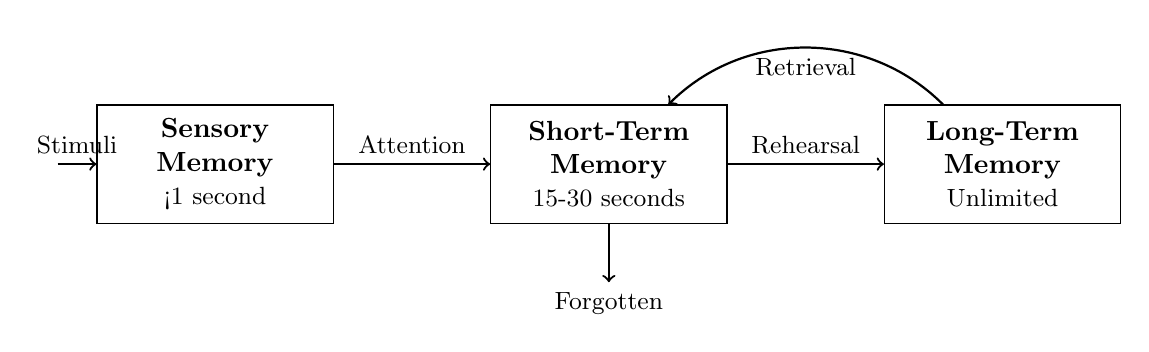
\begin{tikzpicture}[
    box/.style={rectangle, draw, minimum width=3cm, minimum height=1.5cm, align=center},
    arrow/.style={->, thick}
  ]
    % Boxes
    \node[box] (sensory) at (0,0) {\textbf{Sensory}\\\textbf{Memory}\\{\small <1 second}};
    \node[box] (stm) at (5,0) {\textbf{Short-Term}\\\textbf{Memory}\\{\small 15-30 seconds}};
    \node[box] (ltm) at (10,0) {\textbf{Long-Term}\\\textbf{Memory}\\{\small Unlimited}};

    % Arrows
    \draw[arrow] (sensory) -- node[above] {\small Attention} (stm);
    \draw[arrow] (stm) -- node[above] {\small Rehearsal} (ltm);
    \draw[arrow] (ltm) to[bend right=45] node[below] {\small Retrieval} (stm);

    % Input/Output
    \draw[arrow] (-2,0) -- node[above] {\small Stimuli} (sensory);
    \draw[arrow] (stm) -- +(0,-1.5) node[below] {\small Forgotten};
  \end{tikzpicture}
  \end{center}

  \vspace{1em}

  \textbf{Key Processes:}
  \begin{itemize}
    \item \textbf{Attention} - Moves information from sensory to short-term
    \item \textbf{Rehearsal} - Transfers information to long-term storage
    \item \textbf{Retrieval} - Brings stored information back to working memory
    \item \textbf{Forgetting} - Information lost at each stage without processing
  \end{itemize}
\end{frame}

\begin{frame}
  \frametitle{Why This Model Matters}

  \textbf{Scientific Impact:}
  \begin{itemize}
    \item Unified many findings about memory
    \item Generated decades of testable predictions
    \item Foundation for modern memory research
  \end{itemize}

  \vspace{1em}

  \textbf{Practical Applications:}
  \begin{itemize}
    \item \textbf{Education} - Spaced repetition and rehearsal strategies
    \item \textbf{Design} - Understanding cognitive load in interfaces
    \item \textbf{Clinical} - Diagnosing memory disorders
  \end{itemize}

  \vspace{1em}

  \textbf{Modern Updates:}
  \begin{itemize}
    \item Working memory is more complex than originally thought (Baddeley)
    \item Multiple long-term memory systems (procedural, episodic, semantic)
    \item But the basic framework still holds
  \end{itemize}
\end{frame}

% ============================================================================
% YOUR CONTENT SECTIONS GO HERE
% ============================================================================

% Example slide structure:
% \begin{frame}
%   \frametitle{Slide Title}
%
%   Your content here
%
% \end{frame}

% ============================================================================
% BACKUP SLIDES (optional)
% ============================================================================

% \appendix

% \begin{frame}[allowframebreaks]{References}
%   \printbibliography
% \end{frame}

\end{document}
